\documentclass[../main.tex]{subfiles}

\begin{document}

\subsection{Solution overview}

The proposed solution consists of two main sections: a drone and a monitor section. The user will import or choose 
the mobility pattern and set the constraints to the monitor device, which is a laptop. Then the laptop will send high-level commands to the drone agent, which will apply certain operations such as start/stop etc. Once the user finishes importing the mobility pattern and starting the drone mission, the drone will begin to take off and begin to visit the area to scan for getting the most number of mobile targets using \gls{drl} model. Users will keep receiving live updates and the status of service on the control section using Wi-Fi. Most of the connections in the system are wireless, which will have benefits and drawbacks which will be discussed in hardware/software to be used section.


\subsection{High level architecture}
Figure 1 shows a high-level architecture of a complete working system, in which a group of connected adapters and devices are combined into a single functional system.In the next section, hardware and software details will be presented in a more detailed way.
\begin{figure}[H]
	\centering
	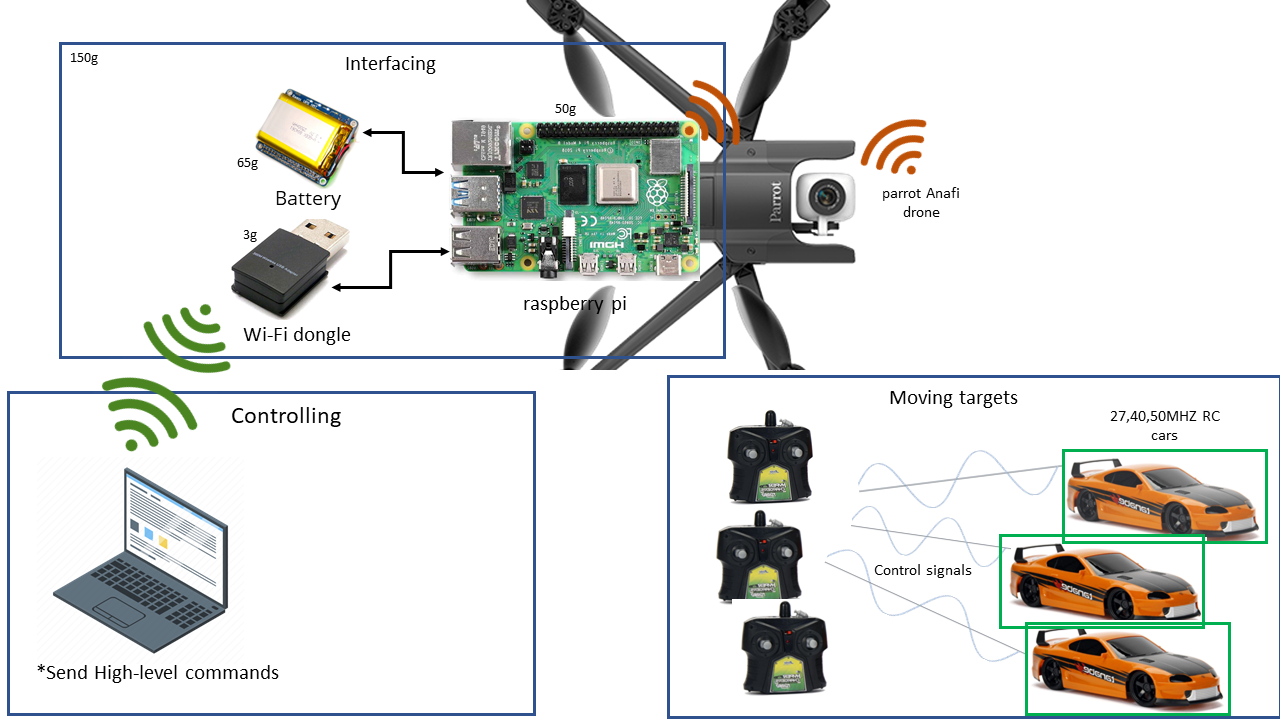
\includegraphics[width=0.9\textwidth]{high-level-arch.png}
	\caption{High-Level Architecture}\label{fig1:arch-fig}
\end{figure}


\subsection{Hardware/software to be used}

\subsubsection{Software}
%parrot olympe
%parrot sphinx
%Gazebo simulator
%roboflow
%google colab notebook /jupyter notebook
The software section contains three primary parts simulation, training, and application. The first part will focus on simulating the environment, testing the models, and flight control. Before discussing the software to be used, we will use the operating system, the base for our software applications. We selected Ubuntu 18.04 operating system for several reasons. One key reason is the compatibility because parrot Olympe and Sphinx are only supported on limited distributions and operating systems. Another reason its a lite os and can be installed on the onboard computer that will be attached to the drone.For the simulation part, using Sphinx and gazebo software is very helpful in visualizing the environment and how drone flight and apply the model.[more talk about simulation].In the training part, we used the simulation tools to generate some training datasets. We use a website called roboflow which helped us labeling the objects and generate new datasets from the existing ones with modified constraints like rotation and scaling. For the object detection model, google colab notebook was a sufficient tool to start training using \gls{cnn} Yolov5.[more talk about roboflow/training].Application software used in this project was parrot Olympe to send commands to the drone and control the flight trip and how the drone moves.[more talk about application software].


\subsubsection{Hardware}
%Parrot ANAFI Drone
%Raspberry Pi 4
%lithium Battery
%Wi-Fi adapter dongle
%laptop control station
python script. Good flight time support, ANAFI drone has a 2700mAh battery which can fly up to 25 min which is good enough in our application. Finally, the support of Wi-Fi 802.11 and \gls{gps} features is essential in our project. The second important device is the Raspberry Pi which will be used as an onboard computer and will handle several tasks—connecting to the drone using a Wi-Fi interface. Controlling the drone by executing the python scripts to send/receive fly control instructions to the drone. Apply the machine learning and \gls{drl} models, which will be synchronized with the control part.Send/receive high-level commands and results to the laptop/pc ground station. It is connected using another 2.4GHz Wi-Fi interface with the help of a Wi-Fi adapter dongle connected to the Raspberry Pi through USB. The power source for the Raspberry Pi will be a lithium battery with the power board will be attached to the board, and its 4000mAh lithium battery will provide enough power and time for our application.      

\end{document}
